\clearpage\null\newpage
\section{Sviluppo}
Lo sviluppo del software per la gestione della PadovaCard è stato fatto seguendo le specifiche progettuali descritte nella Sezione \ref{specificacomponenti}.
Gli strumenti di lavoro utilizzati sono desritti nella Sezione \ref{strumentidilavoro}.
\subsection{Documentazione del codice}
La documentazione del codice è stata in parte automatizzata con l'utilizzo di PHPDocumentor, che genera la documentazione partendo da tag inseriti nel codice sorgenti.
Questi tag sono inseriti a livello di controller, quindi all'inizio di ogni file, per descrivere il suo scopo e il suo ruolo all'interno della struttura \glossario{MVC}, quindi a livello di metodo per descrivere nel dettaglio cosa fa il metodo, quali parametri prende in input e quali dati ritorna.
Tali tag vanno inseriti all'interno di speciali campi commento, obbligatoriamente sopra il metodo che descrivono. \\

Grazie ad un apposito plugin per Sublime text 3, l'IDE utilizzato, è stato possibile velocizzare la scrittura dei tag grazie ad un autocomletamento intelligente. Con l'aiuto di un altro plugin è stato possibile ottenere suggerimenti sui metodi durante il loro utilizzo, mediante una funzione simile ad \glossario{IntelliSense}.
Di seguito un esempio dei tag 
\lstset{frame=single}
\begin{center}
\begin{lstlisting}
/**
 * view method
 *
 * Questo metodo ritorna i dati di un singolo utente assieme alle caratteristiche del gruppo di appartenenza
 *
 * @throws NotFoundException
 * @param string $id
 * @return void
 * @package UsersController
 */
\end{lstlisting}
\end{center}
Mano a mano che i metodi sono stati creati o modificate venivano creati anche i tag, cosi facendo in ogni momento è possibile lanciare dalla \textit{root} del software il comando
\textit{phpdoc run -template "clean"} per ottenere un file html contenente la documentazione.
Di seguito un esempio della documentazione ottenuta.

\begin{figure}[H]
\centering
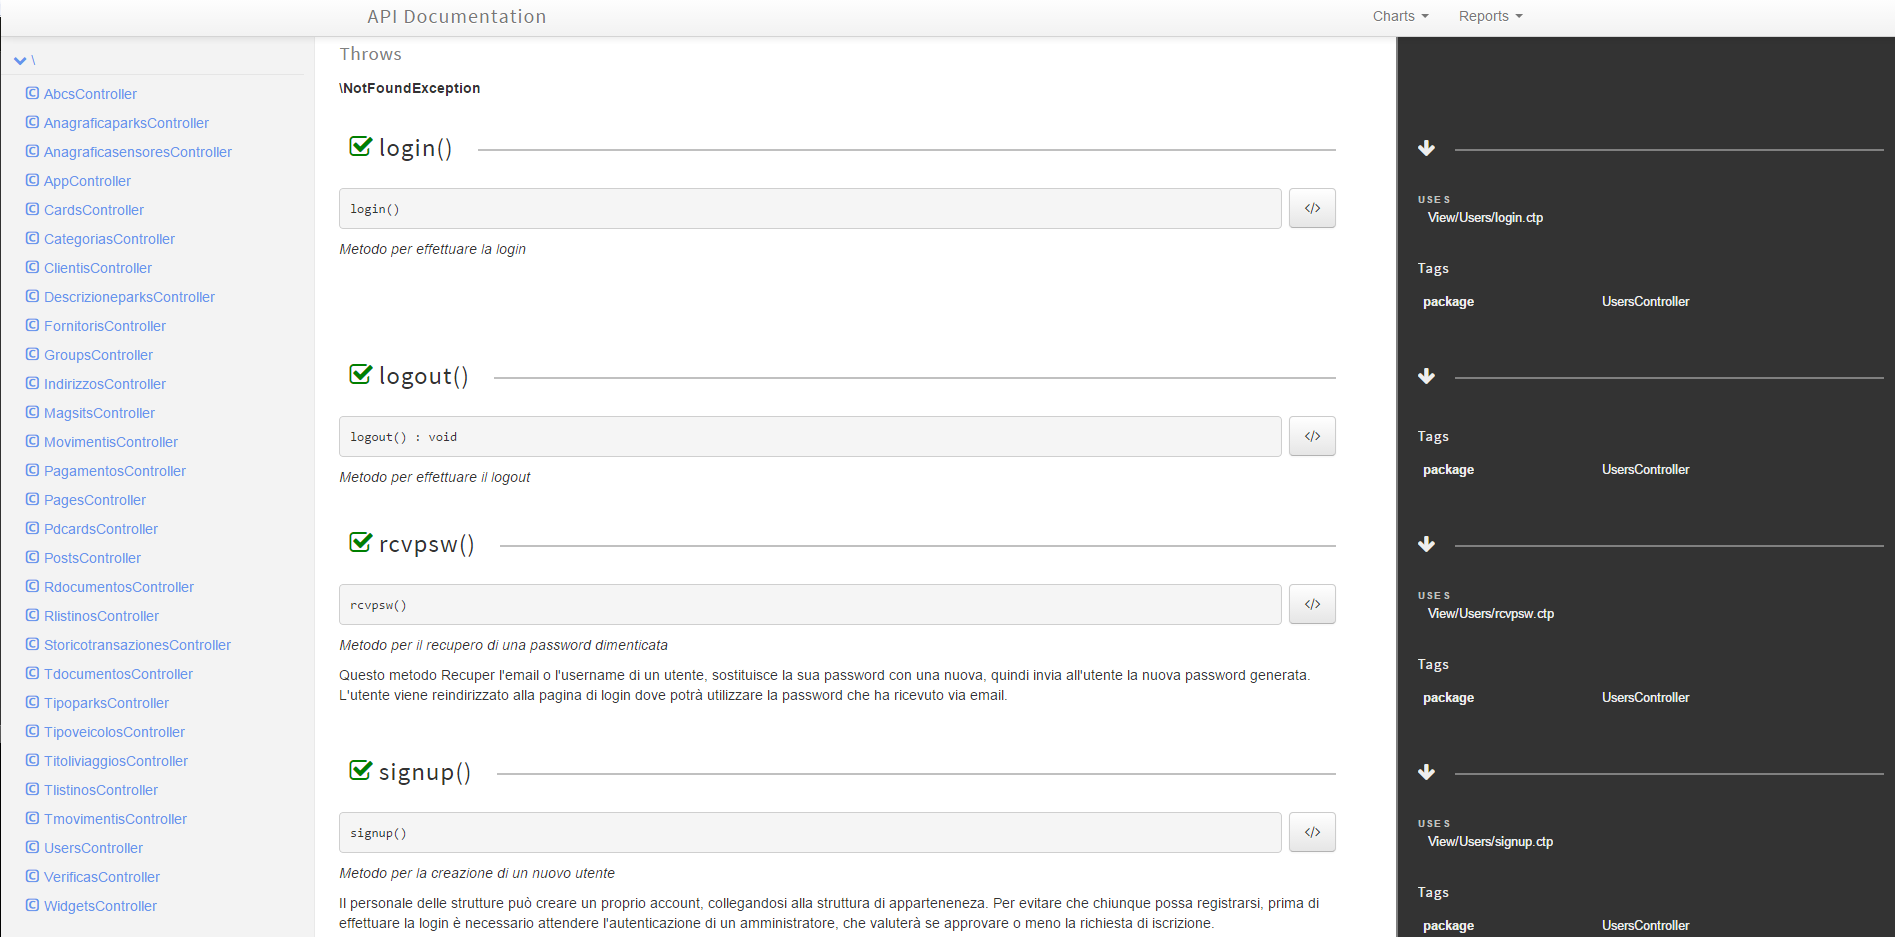
\includegraphics[width=1.2\textwidth]{images/phpdocumentor.png}
\caption{Esempio di documentazione ottenuta con PHPDocumentor}
\end{figure}

In azienda esiste una wiki contenente la documentazione di tutti i progetti, questo permette ad ogni sviluppatore di conoscere il funzionamento dei vari software in autonomia. A progetto concluso anche questa documentazione verrà aggiunta alla wiki.

\subsection{Versionamento del codice}
Per il versionamento del codice è stato usato \glossario{CVS} in quanto già presente nel server di staging e sulle macchine degli sviluppatori è stato installato smartCVS, un interfaccia grafica per l'utilizzo di CVS.
Prima di iniziare a lavorare si aggiorna la repo locale con quella remota, quindi si risolvono eventuali conflitti e solo allora si inizia a modificare il codice. Quando una funzionalità è stata implementata e testata in locale la si aggiunge sulla repo, e quindi sul server di staging, infatti la directory utilizzata da apache nel server di staging era diversa dalla repo, questo per problemi di configurazione del server. Si è ritenuto meno time consuming %TODO 
effettuare un doppio caricamento (prima sulla repo e poi sul server) piuttosto che rivedere le configurazioni del server.